% mnras_template.tex 
%
% LaTeX template for creating an MNRAS paper
%
% v3.0 released 14 May 2015
% (version numbers match those of mnras.cls)
%
% Copyright (C) Royal Astronomical Society 2015
% Authors:
% Keith T. Smith (Royal Astronomical Society)

% Change log
%
% v3.0 May 2015
%    Renamed to match the new package name
%    Version number matches mnras.cls
%    A few minor tweaks to wording
%    
%    Beta testing only - never publicly released
%    First version: a simple (ish) template for creating an MNRAS paper

%%%%%%%%%%%%%%%%%%%%%%%%%%%%%%%%%%%%%%%%%%%%%%%%%%
\documentclass[usenatbib]{mnras}
%\usepackage{newtxtext,newtxmath}
\usepackage[T1]{fontenc}


%%%%% AUTHORS - PLACE YOUR OWN PACKAGES HERE %%%%%
\usepackage{graphicx}	% Including figure files
\usepackage{amsmath}	% Advanced maths commands
\usepackage{amssymb}	% Extra maths symbols

%%%%%%%%%%%%%%%%%%%%%%%%%%%%%%%%%%%%%%%%%%%%%%%%%%

%%%%% AUTHORS - PLACE YOUR OWN COMMANDS HERE %%%%%
\newcommand{\vdag}{(v)^\dagger}
\newcommand\aastex{AAS\TeX}
\newcommand\latex{La\TeX}
\newcommand{\Msun}{\,{\rm M}$_{\odot}$\,}
\newcommand{\kms}{\,{\rm km s}\ifmmode ^{-1}\,\else $^{-1}$\,\fi}
\newcommand{\Mpch}{\,{\rm Mpc}\,\ifmmode h^{-1}\else $h^{-1}$\fi}
\newcommand{\kpch}{\,{\rm kpc}\,\ifmmode h^{-1}\else $h^{-1}$\fi}
\newcommand{\kpc}{\,{\rm kpc}\,}

%%%%%%%%%%%%%%%%%%%%%%%%%%%%%%%%%%%%%%%%%%%%%%%%%%
\title[Cosmic web elements and the $\beta$-skeleton]{The four cosmic web
  elements from the $\beta$-skeleton}

% The list of authors, and the short list which is used in the headers.
% If you need two or more lines of authors, add an extra line using \newauthor
\author[J. F. Su\'arez-P\'erez et al.]{
J. F. Su\'arez-P\'erez,$^{1}$\thanks{E-mail: jf.suarez@uniandes.edu.co}
Y. Camargo,$^{2}$ 
X.-D. Li,$^{3}$
and J. E. Forero-Romero,$^{1}$
\\
% List of institutions
$^{1}$Departamento de F\'isica, Universidad de los Andes, Cra. 1 No. 18A-10 Edificio Ip, CP 111711, Bogot\'a, Colombia\\
$^{2}$Departamento de F\'isica, Universidad Nacional de Colombia, Ciudad Universitaria, Bogot\'a, Colombia\\
$^{3}$School of Physics and Astronomy, Sun Yat-Sen University, Guangzhou 510297, P.R.China\\
}

% These dates will be filled out by the publisher
\date{Accepted XXX. Received YYY; in original form ZZZ}

% Enter the current year, for the copyright statements etc.
\pubyear{2020}

% Don't change these lines
\begin{document}
\label{firstpage}
\pagerange{\pageref{firstpage}--\pageref{lastpage}}
\maketitle

% Abstract of the paper
\begin{abstract}
We show how it is possible to infer the environments of the cosmic web
of dark matter using the information of the spatial distribution of
galaxies and a machine learning algorithm. 
Handled the set of galaxies as a set of nodes, we applied the
$\beta$-skeleton algorithm to extract geometrical information like the
number of connections or the average distance by galaxy. 
Using these properties of the distribution of galaxies was probed the
classification trees, random forest and SVM algorithms under different
configurations to find the best set of parameters that makes a good
prediction with the lowest confusion.  
The results show that the local average distance between galaxies on
the $\beta$-skeleton is the most important feature for the prediction
of the cosmic web environment. 
This is a good approximation that will allow us to use these
algorithms to make predictions in observational data.  
\end{abstract}

% Select between one and six entries from the list of approved keywords.
% Don't make up new ones.
\begin{keywords}
cosmic web -- $\beta$-skeleton -- machine learning
\end{keywords}

%%%%%%%%%%%%%%%%%%%%%%%%%%%%%%%%%%%%%%%%%%%%%%%%%%

%%%%%%%%%%%%%%%%% BODY OF PAPER %%%%%%%%%%%%%%%%%%
\section{Introduction}
The galaxy distribution on large spatial scales follows a structured 
pattern commonly know as the cosmic web. 
This web consists of dense spheroidal peaks connected by
anisotropic filaments and walls woven across vast under-dense voids
\citep{Bond1996}. 
This pattern can be interpreted in the context provided by the
$\Lambda$CDM cosmology, whereby initial density fluctuations   evolve
into the present-day large-scale structure through graviational
instability \citep{ZelDovich1970,White1987}.  

The cosmic web evolution can be followed in great detail by studying
DM only cosmological simulations. 
Furthermore, there is a great variety of methods to detect and
classify the cosmic web from these simulations into four different
elements: peak, filament, sheet or void \citep{Libeskind2018}.  
However, cosmic web detection algorithms that find these web elements
starting from dicrete positions describing the galaxy distribution are
less common.
Most of them focuse on some cosmic web elements.
For instance, there is a great variety of void-finders
\citep{Platen2007,Neyrinck2008,Ravoux2020} and filaments-finders
\citep{Novikov2003,Zhang2009,Sousbie2010,Chen2015,Luber2019,Malavasi2020}.   

There are two main approaches to find the four cosmic web elements
from the galaxy distribution.
A first approach directly interpolates galaxy positions
on a grid to process this number density field in the same way as a dark
matter density field \citep{Eardley2015,Alpaslan2016,Tojeiro2017,Shadab2019}. 
This approach has a low compuational cost, is highly uncertain how
accurate are these results with respect to the expected  cosmic web
dark matter distribution. 

The second approach performs the reconstruction of the dark matter around
the observed galaxies.
Most of these algorithms use Bayesian statistics coupled with Monte
Carlo sampling  and N-body
simulations \citep{Jasche2010,Jasche2013a,Bos2014,LeclercqJasche2015,Horowitz2019,Burchett2020}. 
Some others are based on the density distribution around halos that
are associated to galaxy groups \citep{Wang2009,2011MNRAS.417.1303M}.  
This generic approach can provide accurate DM distributions, but can
be very expensive from the computational point of view. 

Recently, Machine Learning (ML) methods have been used to solve the
intermediate problem of finding the four web elements from discrete
tracers \citep{Hui2018}. 
This avoids the uncertain grid interpolation of tracers and the expensive
DM density reconstrution.
Under this approach of supervised ML classification needs a training
dataset (some galaxy properties), the classes to classify the dataset
(the four cosmic web environments) and an algorithm capable to link
he galaxy properties to the cosmic web environment.
This paper is inscribed into that line of work.


We want to explore to what extent graph properties built on a galaxy
distribution can predict the cosmic web element to which every galaxy
belongs. 
We demonstrate an specific implementation of this approach by using
the $\beta$-skeleton graph \citep{Fang2019} and the  T-web
\citep{Forero-Romero2009} classification into four cosmic web
elements.  
We test three different supervised machine learning
algorithms (support vector machine, Tree Classifier, Random Forest) 
to train from the features and predict the environment.
We quantify the precision and accuracy of the algorithms using 
the Illustris-TNG simulation \citep{Nelson2015} at redshift $z=0$.

This paper is organized as follows. 
In Section \ref{sec:init} we describe the relevant aspects of the Illustris-TNG
simulations relevant to our work, the T-web algorithm,
and the $\beta$-skeleton graph.
In Section \ref{sec:link} we describe the mechanism to link the
$\beta$-skeleton to the T-Web using machine learning algorithms. 
There we detail the features and meta-parameters we use, the
classification algorithms and the metrics for model evaluation.  
In the Section \ref{sec:results} we present our results
to finally summarize our conclusions in Section
\ref{sec:conclusions}. 


\section{Initial Algorithms and Simulations}\label{sec:init}

\begin{figure*}
\centering
 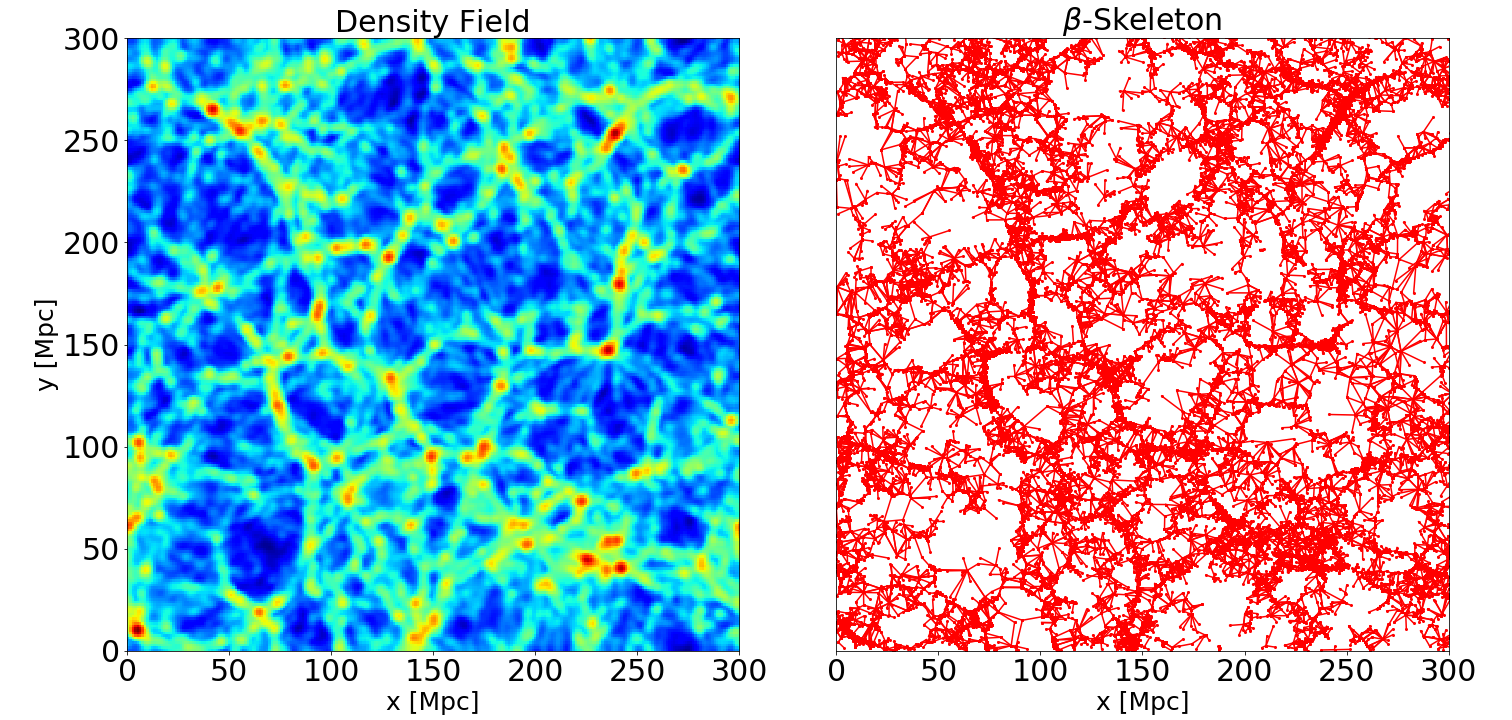
\includegraphics[scale=0.28]{Figs/Fig1_.png}%Figs/p_TWeb_bsk.pdf}
 \caption{Comparison between the T-Web of dark matter density field (left) and the $\beta$-skeleton (right) computed from the distribution of galaxies with $\beta$=1 for Illustris-TNG300.}
 \label{fig:TWebBsk}
\end{figure*}

\begin{figure*}
        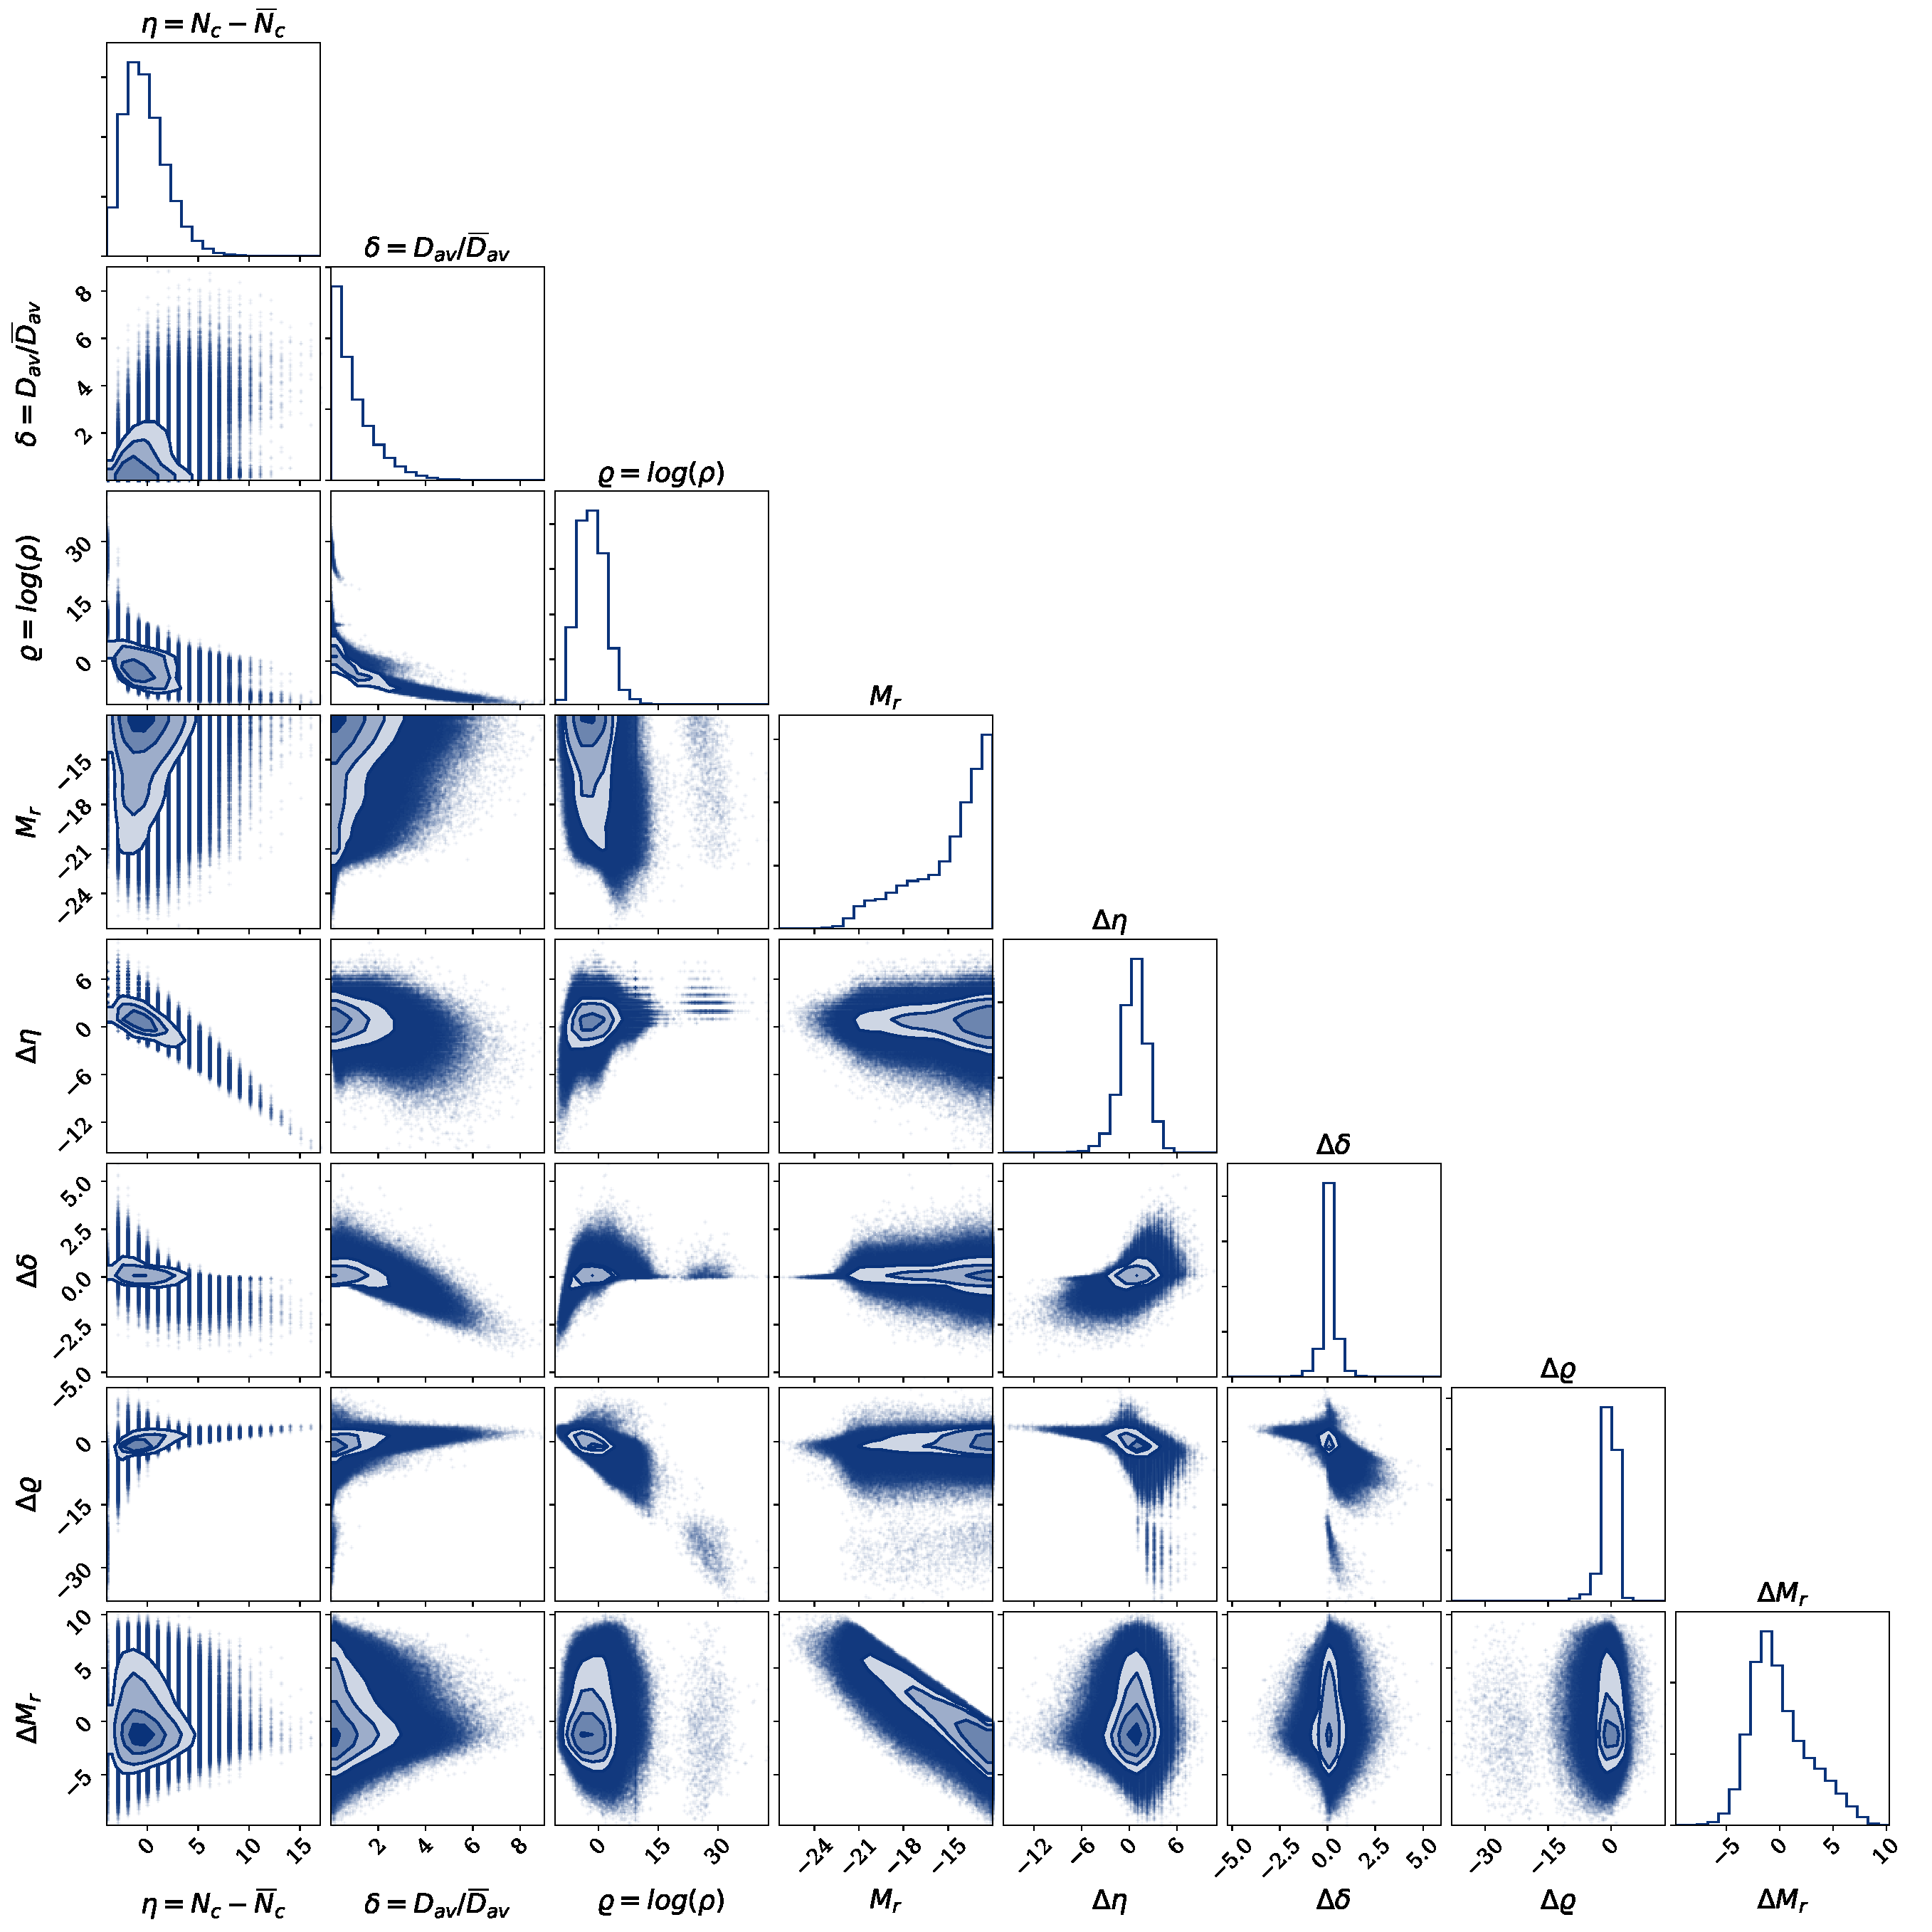
\includegraphics[scale=0.3]{Figs/p_all_features_correlations.pdf}
    \caption{Histograms and correlations curves for the eight features used to train the classifiers.}
    \label{fig:features}
\end{figure*}

\subsection{Illustris-TNG}

The Next Generation (TNG) of the Illustris simulations, or the
Illustris-TNG project \citep{Nelson2015},  is a series of large,
cosmological magnetohydrodynamical and semi-analytical simulations of
galaxy formation. 
These simulations are based on the cosmological standard model
$\Lambda$CDM.  

The Illustris-TNG project simulates different structures in the
visible matter like stars, black holes or diffuse gas jointly with the
distribution of DM.   
The project includes simulated galaxies as realistic as possible in
order to make a comparison with the real universe. There are 18
different simulations in this project with boxes of sizes 50, 100 and
300 Mpc that started at $z=127$ and finalized at $z=0$.   

\subsection{T-Web Classification}

The tidal web (T-Web) method \citep{Hahn2007,Forero-Romero2009}
classifies the large scale structure into four web types: voids,
sheets, filaments and peaks.   
This classification is based on the eigenvalues of the deformation
tensor $T_{\alpha\beta}$, the Hessian of the gravitational potential 
\begin{equation}
T_{\alpha\beta}=\frac{\partial^2\psi}{\partial r_{\alpha}r_{\beta}},
\end{equation}
%
where $\psi$ is a normalized gravitational potential that follows the equation
\begin{equation}
    \nabla^2 \psi = \delta,
\end{equation}
%
and $\delta$ is the dark matter overdensity.
This tensor has three real valued eigenvalues. 
The cosmic web environment is defined by the number of eigenvalues
larger than a threshold value $\lambda_{th}$.
Locations with three eigenvalues larger than $\lambda_{th}$ correspond
to a peak, two to a filamet, one to a sheet and zero to a void. 

Computationally speaking, to define an environment in an N-body
simulation we implement the following seven steps: 1) interpolate the
mass particles with a Cloud-In-Cell  (CIC) scheme over a grid to
obtain the density, 2) smooth it with an isotropic Gaussian filter,
3) compute the overdensity, 4) find the normalized potential with Fast
Fourier Transform  methods, 5) compute the deformation tensor using
finite differences, 6) find the eigenvalues and finally 7) count the
number of eigenvalues larger than the threshold $\lambda_{th}$. 


\subsection{The $\beta$-skeleton algorithm}

The $\beta$-skeleton is an algorithm that computes a graph over a
distribution of nodes \citep{Kirkpatrick1985, Fang2019}.  
This algorithm depends on a positive and continuous parameter $\beta$
that defines an exclusion region between two nodes.
If the exclusion region is empty then, the two nodes are connected by
an edge.  
In the case, $\beta=1$, the exclusion region is a sphere with a
diameter equal to the separation between the two nodes.  

As $\beta$ increases the exclusion region is larger.
This makes that for low values of $\beta$ the graph is dense and for
large values of $\beta$ the graph becomes sparse. 
The $1$-skeleton also receives the name of Gabriel Graph.  
The $2$-skeleton is also known as the Relative Neighbor Graph (RNG). 

In our case, the galaxies represent a node in the graph.
From this graph, we compute a variety of features to be used as
an input for the classification task. 

\section{Linking the $\beta$-skeleton to the T-Web}\label{sec:link}



Figure \ref{fig:TWebBsk} shows the correlation between the DM overdensity
and the $\beta$-skeleton graph computed over the corresponding galaxy
distribution. 
This spatial correlationsuggests that graph derived features might have
a good chance to predict the DM web environment. 
However, there is a number of free parameters that have to be explored
to find the best match between the $\beta$-skekeleton and the cosmic
web.


\subsection{T-web and $\beta$-skeleton free parameters}

For a start, the influence of the $\beta$ parameter has to be explored.
Additionally, the classification provided by the T-web algorithm
depends on the smoothing scale, $\sigma$, used to compute the Hessian and the
threshold parameter $\lambda_{th}$ used to define the web elements.
The tracers we use from the simulation can also change. 
We use a simple magnitude cut $M_{th}$ on the $r$-band absolute magnitudes
to define the galaxy sample. 
Different values for that threshold naturally produce different galaxy
distributions and thus different $\beta$-skeletons. 

For given values of these four different parameters ($\beta$,
$\sigma$, $\lambda_{th}$ and $M_{th}$) the $\beta$-skeleton and the
T-web are fixed.
Next we define what features to use to predict the four cosmic web
elements. 

\begin{figure*}
  \centering 
    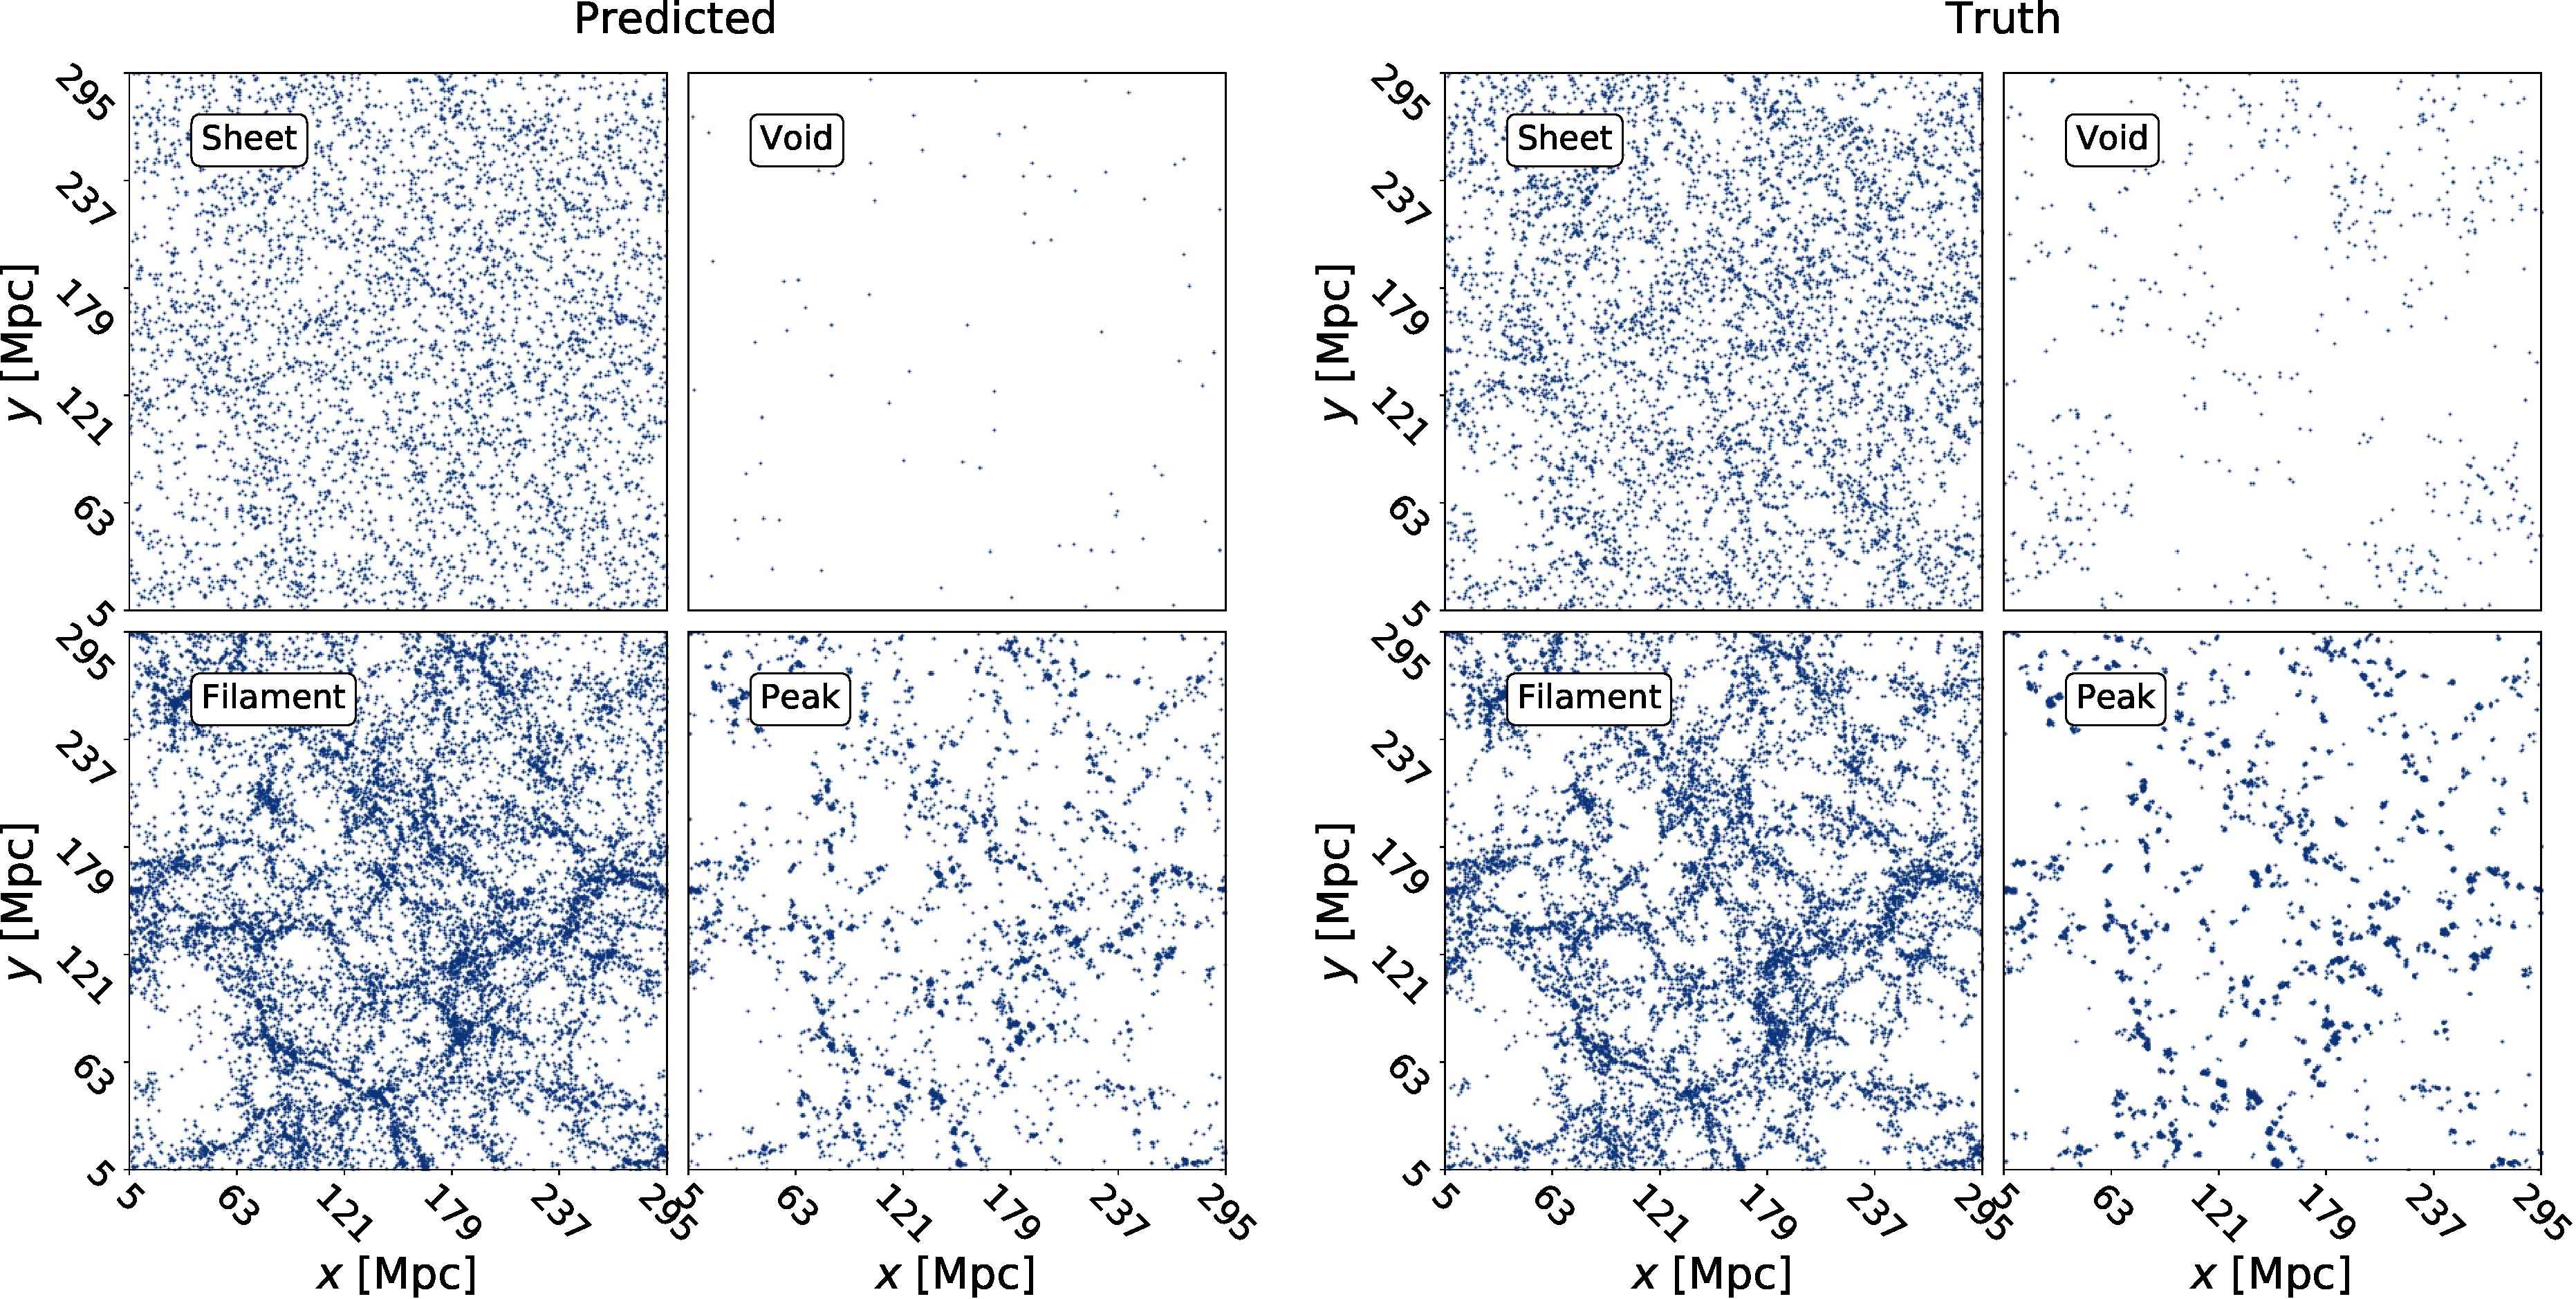
\includegraphics[scale=0.32]{Figs/p_environment_predicted.pdf}
    \caption{Comparison between the DM T-Web from the Illustris-TNG
      simulation and the environments predicted by the Tree Classifier
      algorithm.} 
    \label{fig:prediction}
\end{figure*}

\subsection{Features and meta-parameters}

We use eight features to train the classifiers.
Six features come from the $\beta$-skeleton algorithm applied over the distribution
of galaxies with $\beta=1$.
The first parameter is the number of connections minus the overall average number of
connections, $\eta = N_c - \bar{N}_c$. 
The second parameter is the ratio between the average distance across neighbors and its median
value over all galaxies in the simulations $\delta=D_{av}/\bar{D}_{av}$.
The third parameter is the logarithm of the pseudo-density $\rho$, $\varrho$. 
This pseudo density $\rho$ is defined as the inverse of the volume computed from the ellipsoid that best fits the distribution of graph neighbors.
We define three more features that we call $\Delta$-features: $\Delta\eta,\Delta\delta\,\text{and}\,\Delta\varrho$. 
These values are computed as the difference between the corresponding value in a node and the 
average value over first neighbors nodes.
Two more features come from the simulation. The absolute magnitude in the 
$r$-band, $M_r$, and its corresponding $\Delta M_r$.
Figure \ref{fig:features} shows the histogram for all $\beta$-skeleton features.

We also use the threshold $\lambda_{th}$ and the smoothing parameter $\sigma$ as
meta-parameters that drive the T-Web classification. 
We take $\lambda_{th}=0.0, 0.1, 0.2, 0.3, 0.4$ and $0.5$.
For the smoothing parameter we take the values $\sigma=0.5$, $1.0$, $1.5$, $2.0$ and $2.5$. 


\subsection{Classification Algorithms}

We applied three different supervised machine learning algorithms: support vector machine (SVM),
classification trees and random forests as implemented in scikit-learn. 
 For each algorithm we explore the following metaparameters:
\begin{itemize}
    \item SVM: 
        \begin{itemize}
            \item $kernel$: \textit{rbf} or Radial basis function
            \item \textit{Max. iterations}= 500,1000,1500,2000,2500.
        \end{itemize}
    \item Classification trees
        \begin{itemize}
            \item \textit{Max. depth}: From 1 to 30.
        \end{itemize}
    \item Random forest
        \begin{itemize}
            \item \textit{Max. depth}: 10.
            \item \textit{Number of estimators}: From 1 to 100.
        \end{itemize}
\end{itemize}

\begin{figure*}
    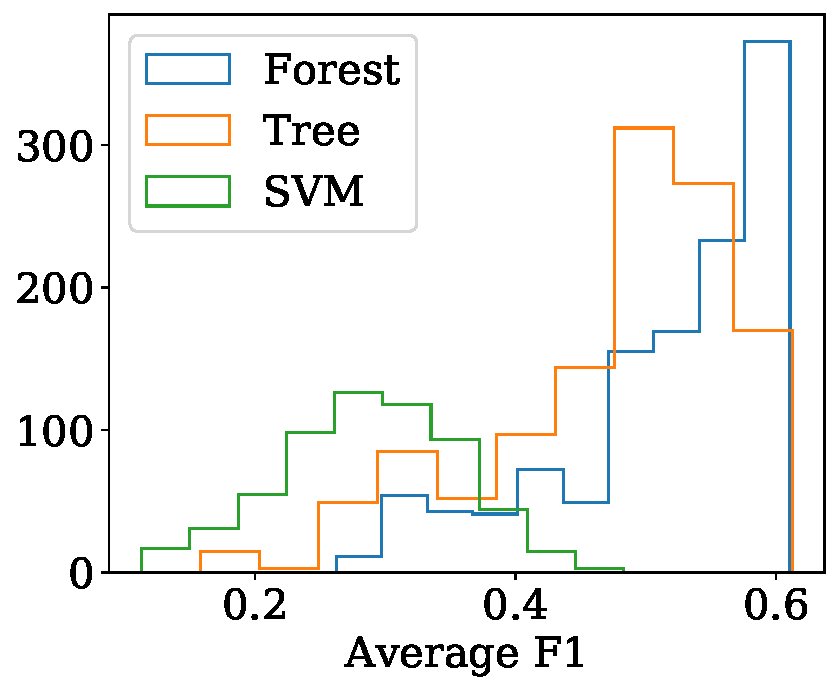
\includegraphics[scale=0.46]{Figs/p_hist_f1.pdf}
    \caption{Distributions of the F1 average for the three machine learning methods. F1-score average distributions considering the four environments (left) and without consider the voids (right).}
    \label{fig:methods}
\end{figure*}







\subsection{Model evaluation}


From the box simulation, we select randomly a 50$\%$ of galaxies by class of environment to train the ML algorithms. We use the other 30$\%$ as test and  20$\%$ as validation. Due to the box simulation has periodic conditions, we selected the galaxies located between 5Mpc and 295Mpc in order to make the model consistent.  
As success metrics, we compute the precision, recall and the F1 score (harmonic mean between precision and recall).
We use the average F1 score across classes to select the best models and its meta-parameters.

\section{Results}\label{sec:results}

\begin{figure*}
    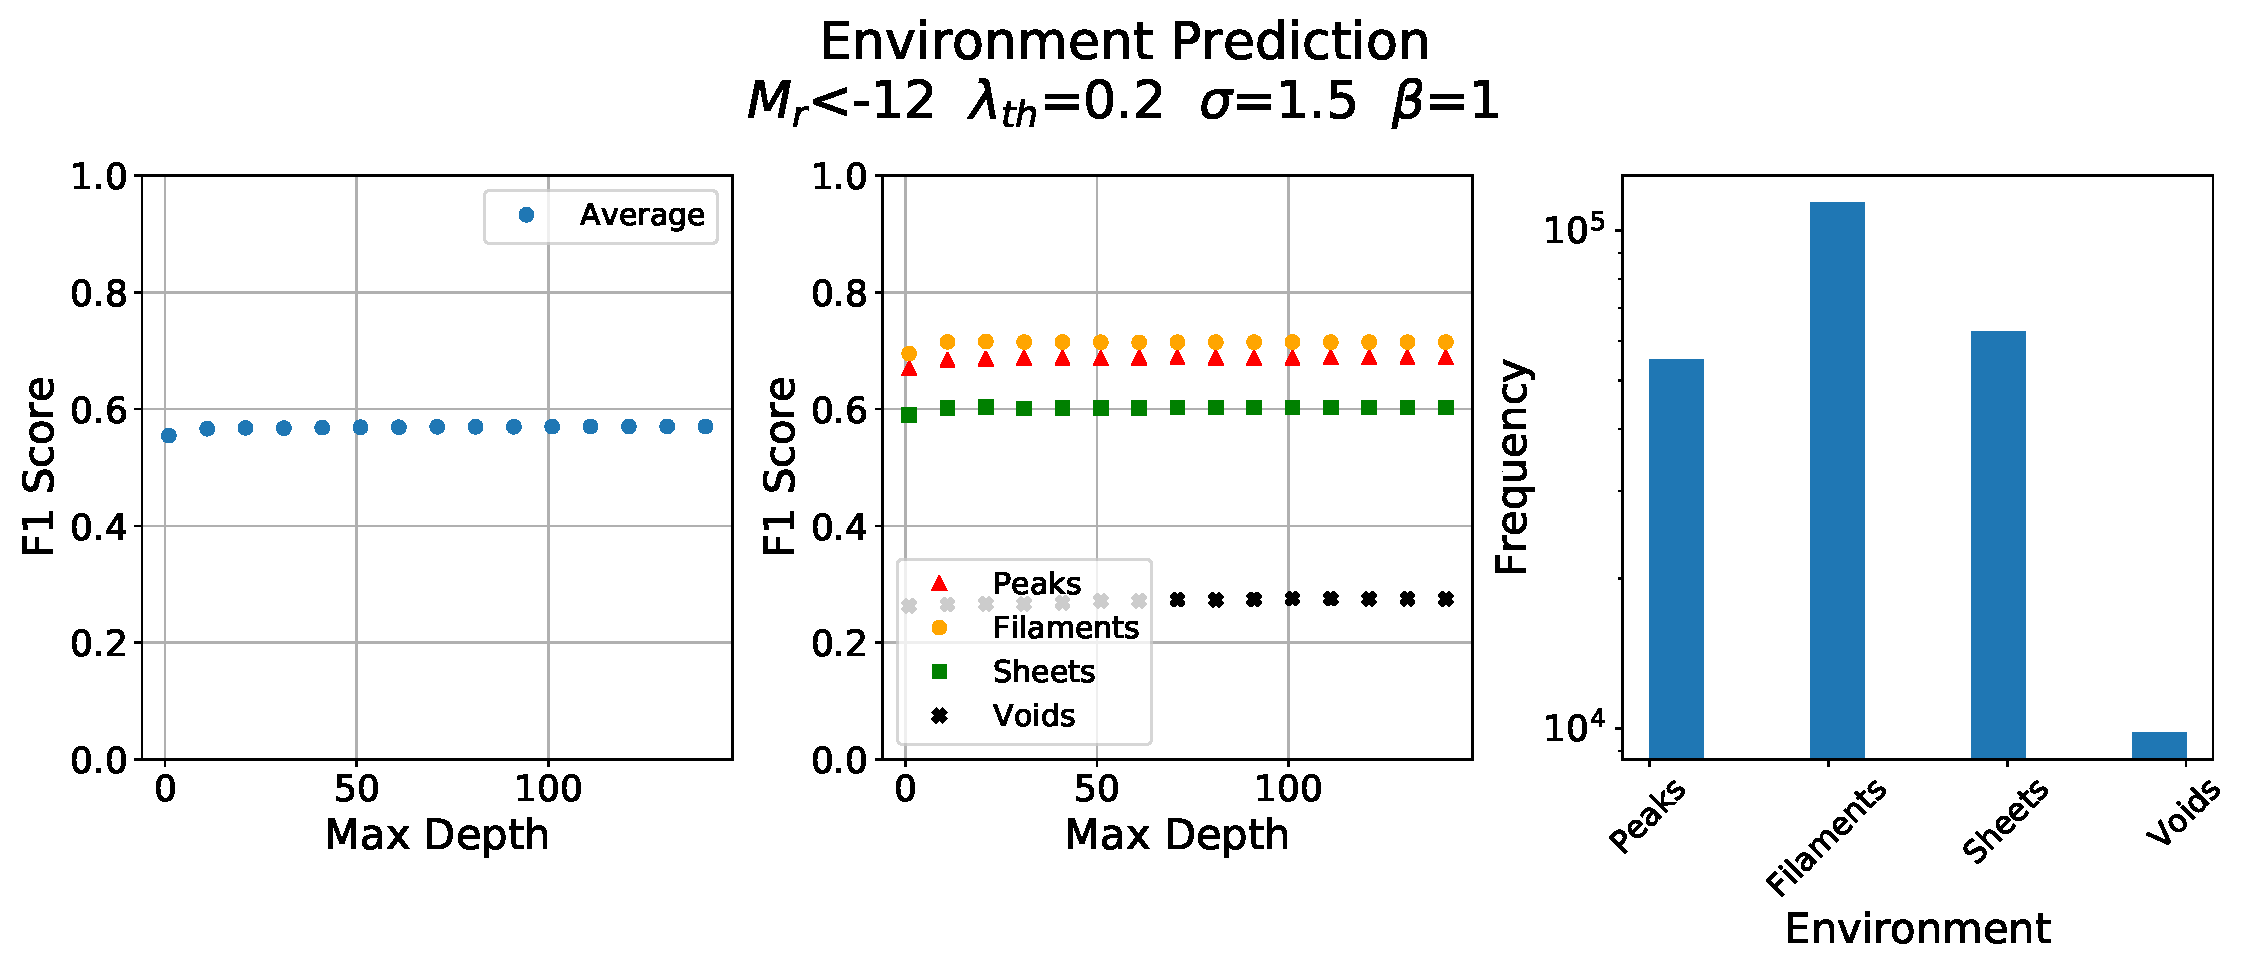
\includegraphics[scale=0.43]{Figs/p_F1_curve_Forest.pdf}
    \caption{The evaluation of the Random Forest algorithm was computed with the F1 score. Here the evaluation of the F1 average score  was computed for $\lambda_{th}=0.2$, $\sigma=1.5$ and $M_r<-12$.  In the left figure was evaluated the F1 average score for the prediction of all environments as a function of the Number of Estimators of the random forest classifier. The center figure show us the evaluation for the prediction by environment, here the best predicted environment are the filaments, for this, the maximum F1 score is near to 0.7. The right figure show the population by environment using to make the prediction with the Random Forest ML algorithm.}
    \label{fig:F1_curve}
\end{figure*}


Figure \ref{fig:prediction} shows the comparison between the ground truth environments (left) and the prediction by the best ML algorithm with the optimized parameters and meta-parameters (right) for the best method.
The visual impression is that the sheets and filaments have good predictions,
peaks are reasonable, while voids are the worst.

\begin{table*}
\centering
\begin{tabular}{cccccccc}
\hline
 Method   & $F1_{peak}$     & $F1_{fila}$     & $F1_{sheet}$    & $F1_{voids}$    & $F1_{av}\,[all]$   & $F1_{av}\,[without \,\,voids]$   \\
\hline
 Forest   & 0.520 $\pm$ 0.261  & 0.716 $\pm$ 0.054 & 0.558 $\pm$ 0.054 & 0.274 $\pm$ 0.187 & 0.517 $\pm$ 0.085  & 0.598 $\pm$ 0.084 \\
 Tree     & 0.468 $\pm$ 0.243 & 0.663 $\pm$ 0.071 & 0.505 $\pm$ 0.104 & 0.272 $\pm$ 0.173 & 0.477 $\pm$ 0.093 & 0.545 $\pm$ 0.089  \\
 SVM      & 0.426 $\pm$ 0.090  & 0.332 $\pm$ 0.095 & 0.266 $\pm$ 0.097 & 0.129 $\pm$ 0.099 & 0.288 $\pm$ 0.068 & 0.341 $\pm$ 0.072   \\
\hline
\end{tabular}
\caption{The Table summarized the results for the 20 best models with the three machine learning methods probed: Random Forest, Tree Classifier, and SVM. It was computed the mean value and error in the F1 score by method in both cases: with voids $F1_{av}\,[all]$, and without voids $F1_{av}\,[without voids]$. According to these results, the best method is the Random Forest algorithm when we do not consider the voids in the F1 average.}
\label{tab:methods}
\end{table*}

The comparison between all results obtained for the three machine learning methods is in terms of the F1 average score. These results are represented in Figure \ref{fig:methods}, when the voids are considered to compute the F1 average (left) and when not (right). 
To evaluate the methods, it was computed the mean values and errors for the 20 larger F1 by method. Table \ref{tab:methods} show mean values for the F1 by environment and the averages considering voids and not.
In general, in both cases, the evaluation show that the best method is the Random Forest. 

The Random Forest have other types of configurable parameters, the most common parameter is the number of estimators NE, we evaluate the Random Forest with the F1 score as a function of the NE parameter. 
Figs.\ref{fig:F1_curve} show the behavior of the F1 average score as a function of NE in contrast to the populations of the environments,
the left figure shows the F1 average score,
the maximum is near to 0.6 for a number of estimators bigger than 15.
The center figure shows the F1 score for the four environments,
the best environment predicted was the filaments followed by the peaks and sheets,
the worst predicted environment was the voids,
this due the population of them as we can see in the right figure of the Fig.\ref{fig:F1_curve},
we can observe that the amount of voids is considerably less than the others environments almost in one order.

\begin{figure*}
\centering
    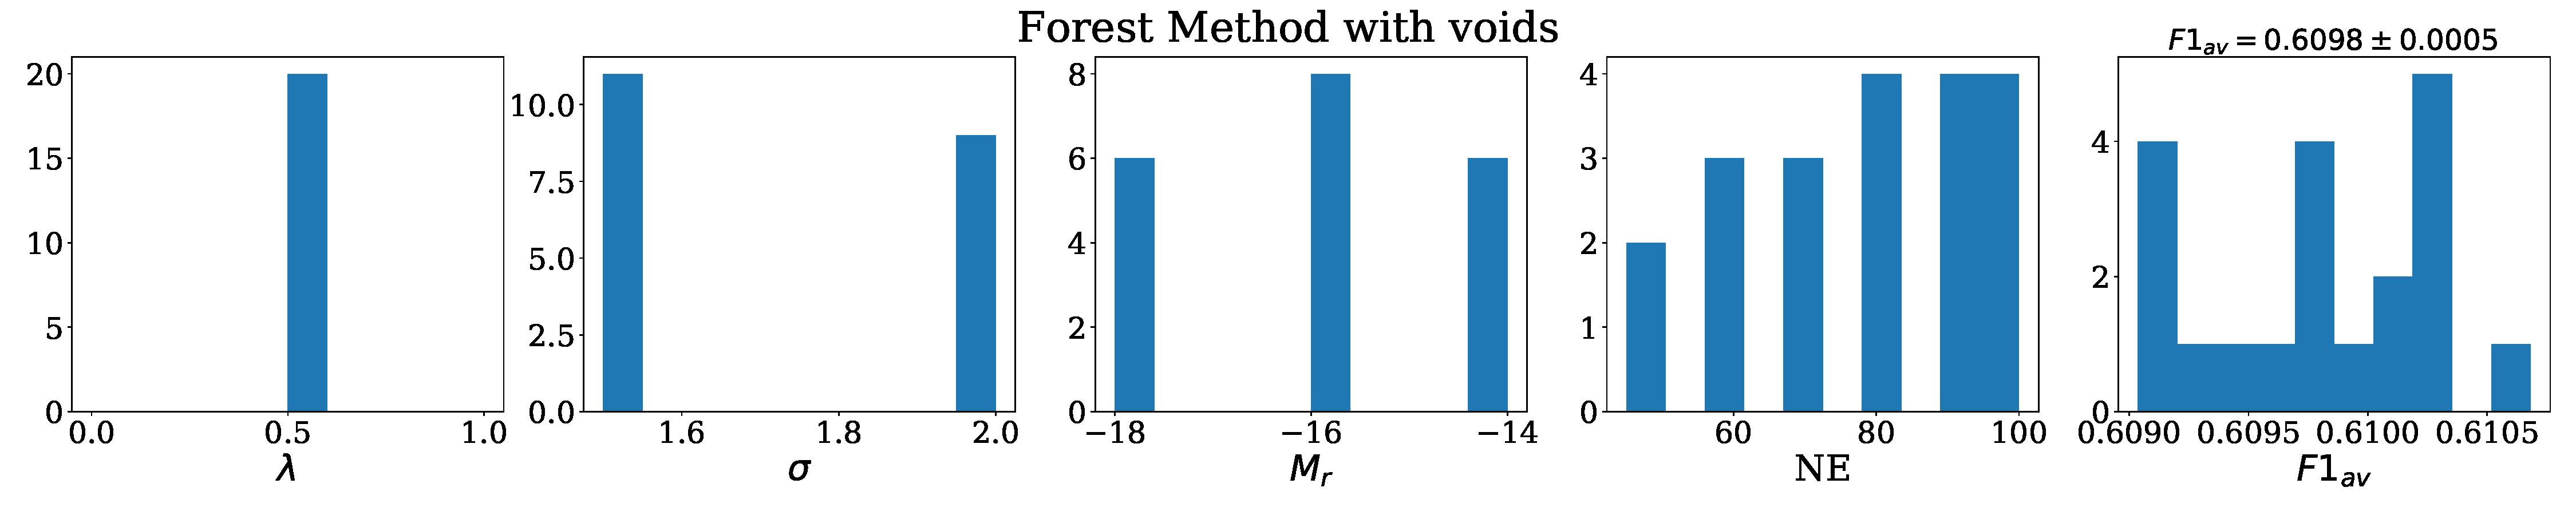
\includegraphics[scale=0.23]{Figs/p_features_Forest_F1_av.pdf}
    \caption{Distribution of the meta-parameters and the F1 average when the voids are including in the average. We can observe that the $\lambda$ meta-parameter are including in 0.5, $\sigma$ jumps between 1.5 and 2.0, $M_r$ could be -14,-16,-18 and $NE$ are concentrate in 100.}
    \label{fig:features_void}    
\end{figure*}

\begin{figure*}
\centering
    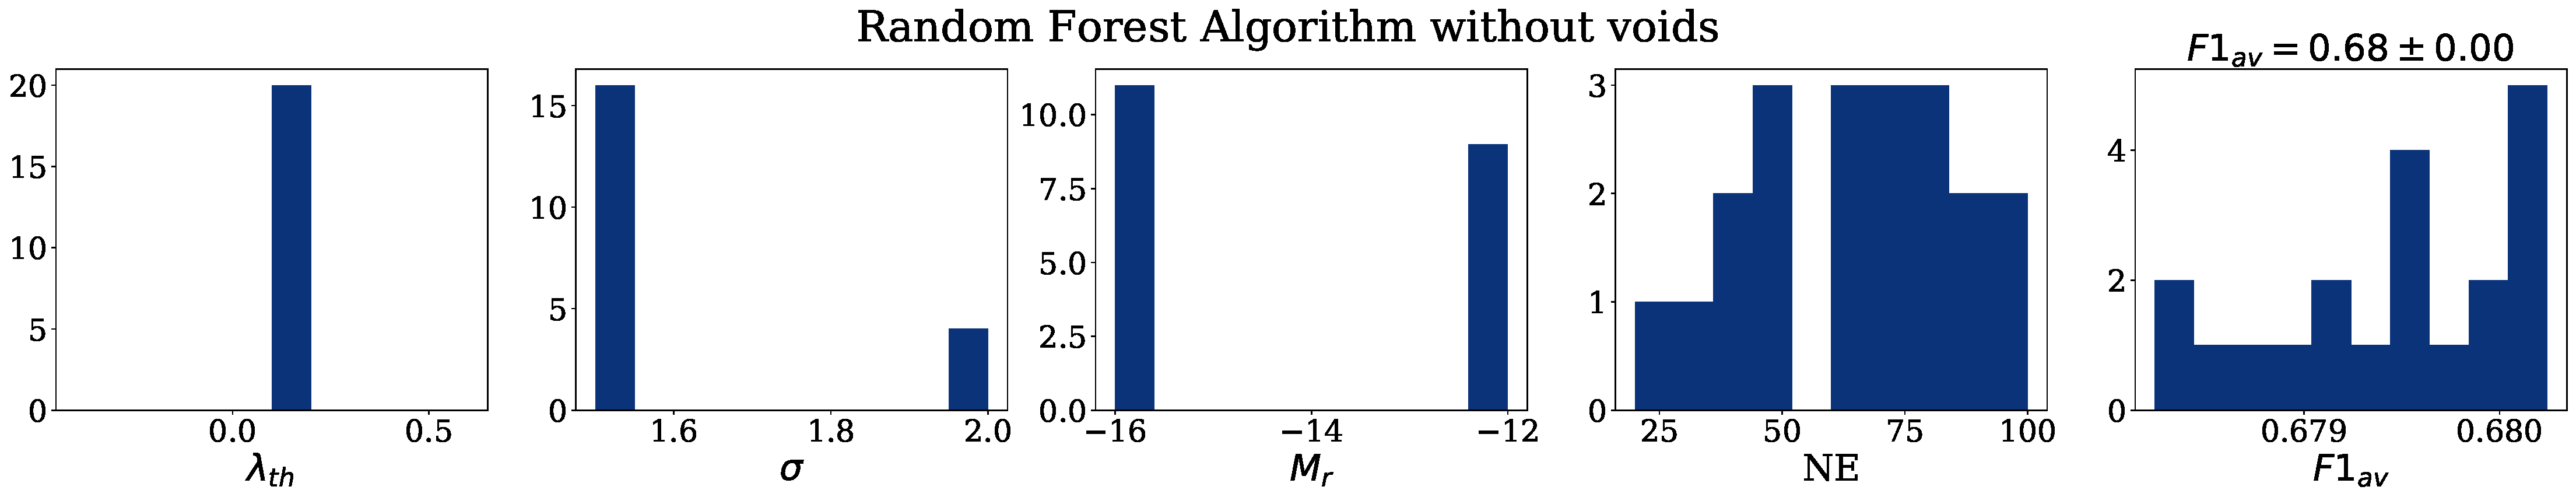
\includegraphics[scale=0.23]{Figs/p_features_Forest_F1_av_no_voids.pdf}
    \caption{Distribution of the meta-parameters and the F1 average when the voids are not including in the average. We can observe that the $\lambda$ meta-parameter is centered in 0.1, mainly, $\sigma$ jumps between 1.5 and 2.0, $M_r$ could be -14 or -16 and $NE$ are concentrate in 80-100.}
    \label{fig:features_no_void}    
\end{figure*}

\begin{figure}
\centering
    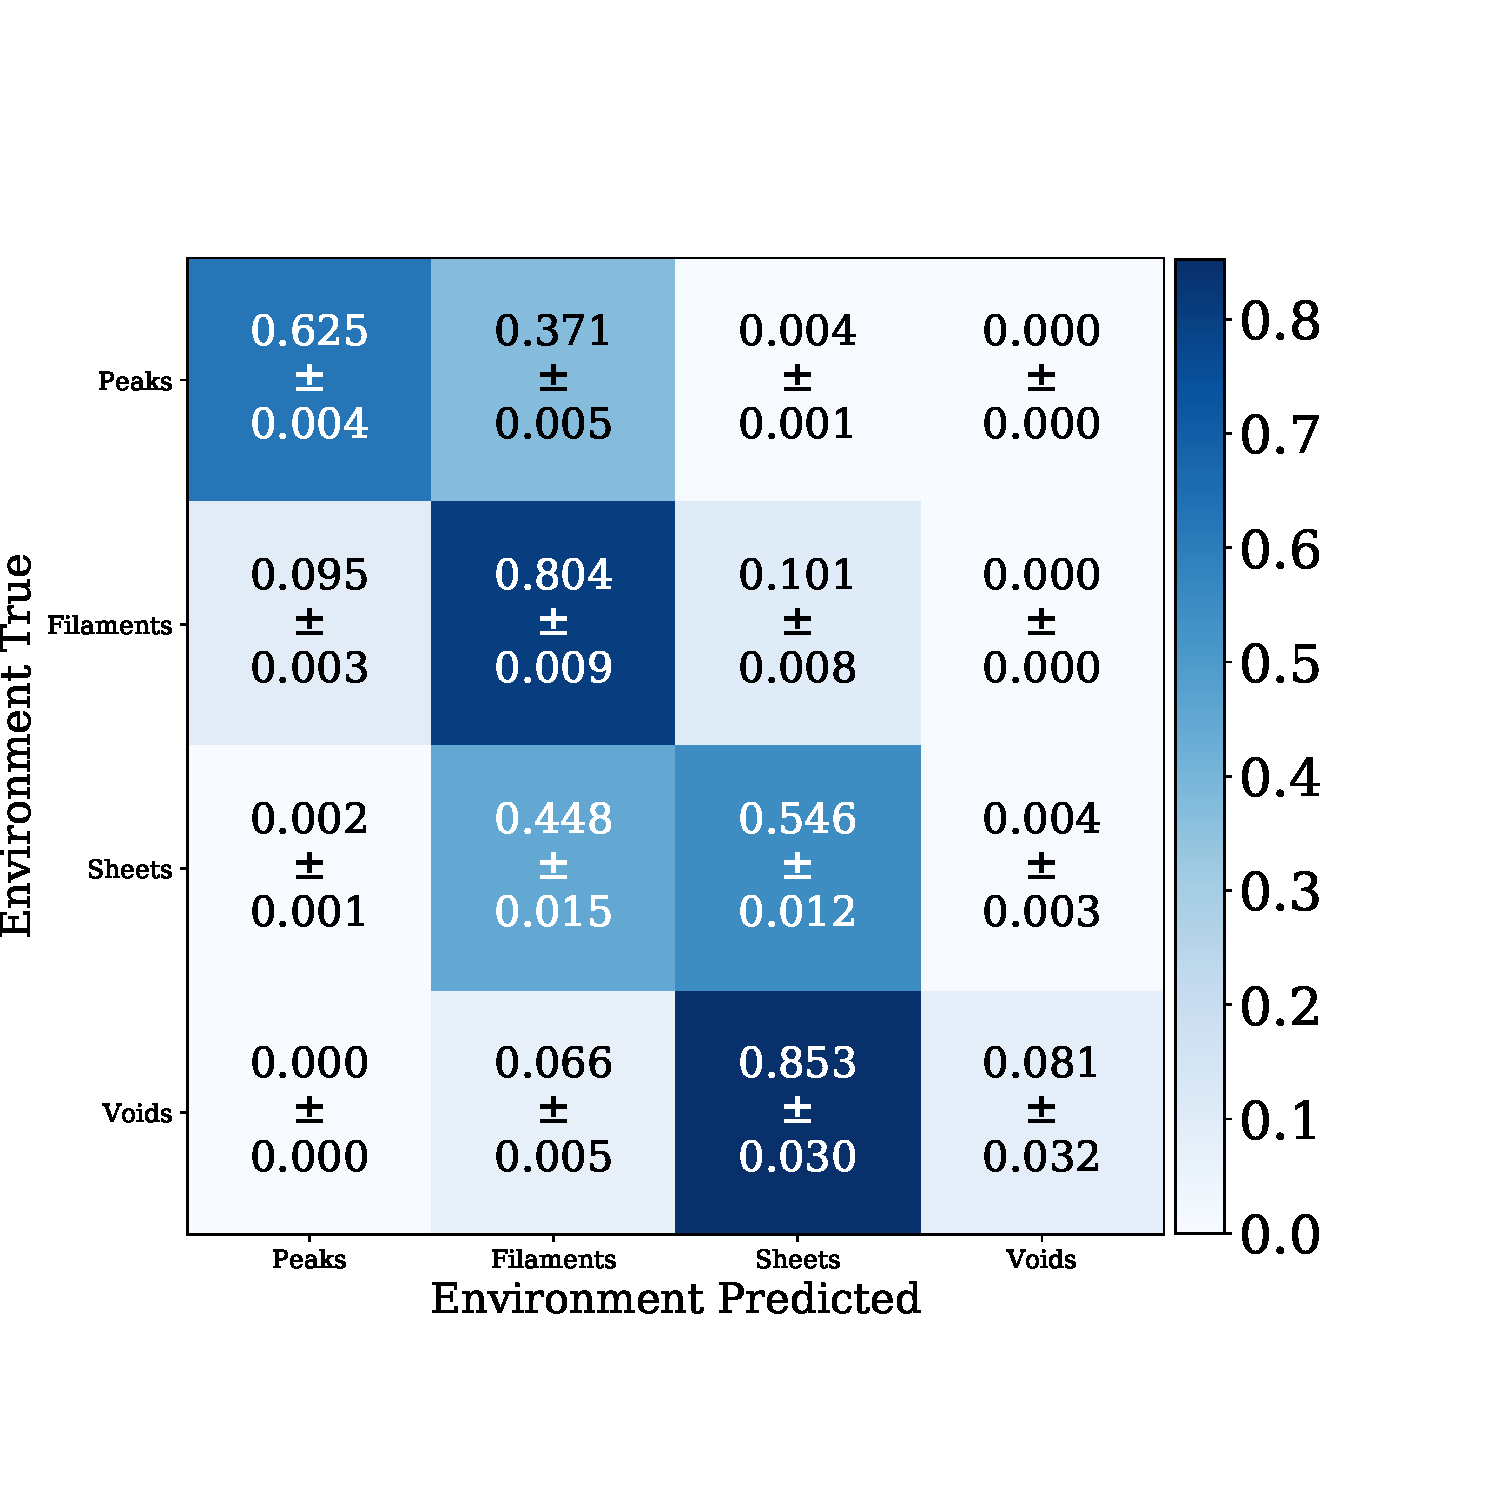
\includegraphics[scale=0.33]{Figs/p_confusion_matrix_20.pdf}
    \caption{Confusion Matrix for the 20 best performing models. Columns represent the predictions, and rows the ground truth. In the CM for the prediction of peaks only the $62\%$ was predicted correctly. The best prediction are obtained for the filaments, where the $80\%$ was predicted correctly. The worst prediction was for the voids where only the $8\%$ was predicted correctly.}
    \label{fig:confusion_matrix}    
\end{figure}

\begin{figure}
\centering
    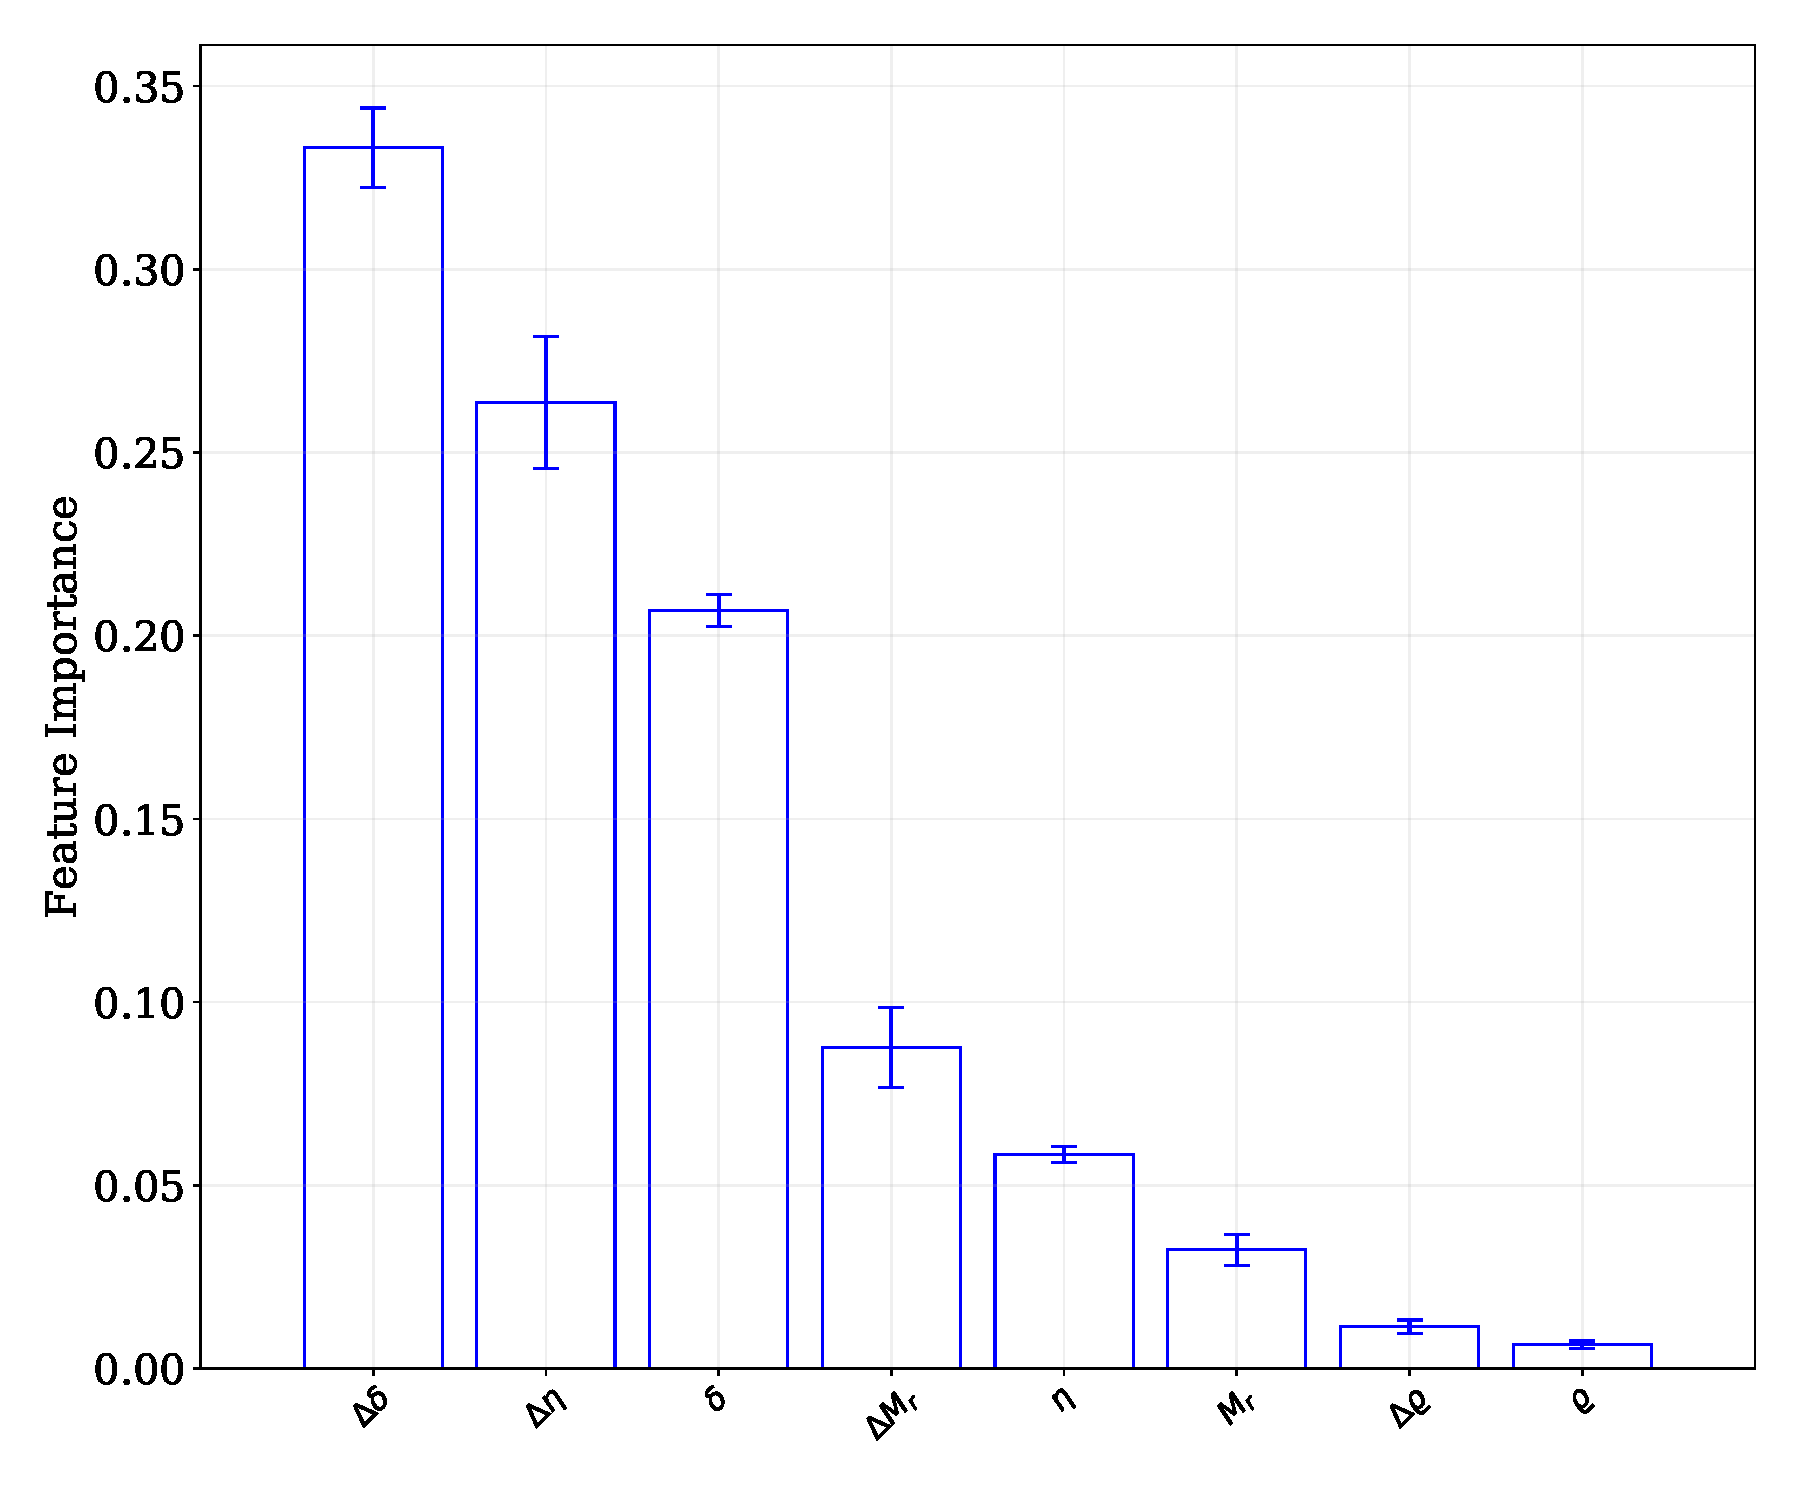
\includegraphics[scale=0.4]{Figs/p_features_importance_20.pdf}  
    \caption{Feature importance for the best classification with $\lambda_{th}$=0.3 ,$\sigma$=1.5, $M_{r}<-14$ and Max Depth=10. This figure show us that the most important variable from the $\beta$-skeleton to make the best prediction are related with the average distance between the connections of the galaxies. The importance of the $\delta$ parameter is near to the $50\%$.}
    \label{fig:feature_importance}     
\end{figure}

Including the NE meta-parameter, the Fig. \ref{fig:features_void} shows the distributions of all meta-parameters for the 20 best results using Random Forest and evaluating the F1 average for the four environments. We can observe that the meta-parameter $\lambda_{th}$ are centered in 0.5 and $\sigma$ have values of 1.5 and 2. For these values of $\lambda$ and $\sigma$, the number of galaxies in voids is not according to reality. Due to this inconsistency, we considered the best 20 results using Random Forest filtering when the F1 average is computed excluding the voids. The distribution of the meta-parameters for this case is shown in Figure \ref{fig:features_no_void}. We can observe in this Figure that threshold $\lambda$ have values of 0.1 and 0.2, the smoothing $\sigma$, 1.5 and 2, and the luminosity $M_r$, -14 and -16. The NE varies between 23 and 100 but is concentrate in values larger than 80.

The bad prediction of the voids illustrated in the Figure \ref{fig:F1_curve} is confirmed by the quantitative results shown in Figure \ref{fig:confusion_matrix} computed for the 20 best models when we do not consider the voids in the F1 average. 

In the Fig. \ref{fig:confusion_matrix} we observe that the best prediction is for filaments where the $80\%$ of the true galaxies in filaments are correctly predicted. 
This fraction is followed by $63\%$ of correct peaks, $55\%$ of correct   sheets galaxies with a low value of $8\%$ void galaxies classified correctly.

Fig.~\ref{fig:feature_importance} shows the importance of the features for the 20 best Random Forests models. According to the Figure, the most important feature for our model is the $\Delta \delta$ feature related to the local average distance between connections, followed by the average distance between connections $\delta$. This Figure shows us that the separation between the galaxies is a parameter that can determinate the T-Web environment for a galaxy. The number of connections is not a relevant parameter to determine the environment due to its importance is not significant.

The best model was evaluated including the information of the features extracted from the 2 and 3-skeleton, the results do not vary in comparison when we used only the features of the 1-skeleton, these showed that the 2 and 3-skeleton do not contain important information to predict the T-Web.


\section{Conclusions}\label{sec:conclusions}

In this paper we presented a method to predict the dark matter cosmic web
environment of a galaxy from its neighbor graph information.
We used the T-web as the cosmic web definition \citep{Forero-Romero2009}
and the $\beta$-skeleton graph \citep{Fang2019} 
to describe the relative spatial distribution of the galaxies. 
The link between the T-web and the graph is done through different
machine learning algorithms: support vector machines, random forests and
classification trees.

We test the method using data from the Illustris-TNG simulation.
The T-web is calculated on a grid of cell size $0.8$\Mpch 
and a Gaussian smoothing scale $\sigma$ and an eigenvalue threshold $\lambda_{th}$.
The $\beta$-skeleton is computed over galaxies brighter than 
an $r$-band absolute magnitude cut $M_{r}$.
For each simulated galaxy we build the $\beta$-skeleton and
compute features such as the number of connections, the average connection
length, the pseudo-density and the difference of these quantities with
respect to the average over first-neighbors.

We find that the T-web environment that is best predicted has smoothing
scale of $\approx1.5$ \Mpch and an threshold $\lambda_{th}=0.3$. 
This turns out to be the ballpark range  favored in previous publications
for T-web  studies for the resulting classification to match the visual impression of the cosmic web \citep{Forero-Romero2009}.
We also find that the features computed with the $1$-skeleton 
(Gabriel Graph) are enough to obtain good predictions. 
The best classification results are not sensitive to the $r$-band
magnitude cut, although a cut of $M_r>-14$ gives the best results.

The best algorithm to predict the environment are the classification
trees followed closely by random forests. 
Support Vector Machines provide the worst results.
From the classification trees we are able to determine that the two most
important features for the environment classification are the average
connection length over the neighbors and the difference of this quantity
with respect to the average over its first neighbors.

The environments that are best predicted are in decreasing order: 
filaments, peaks, sheets and voids. 
This ranking follows the number of galaxies found in each of these environments.
Galaxies in voids represent less that $2\%$ of the total number of galaxies and 
are the hardest class to predict, with $F1$-scores of $\approx0.2$.
Motivated by this limitation, in future work we will present a method to define
voids from the $\beta$-skeleton graph.

All the results we reported here were obtained using a single snapshot at a 
redshift $z=0$.
Our results provide the baseline for future work that will have to quantify 
the effect of redshift space distortions and survey incompleteness in order to
predict  the DM T-Web form survey data.
Nevertheless, the two most interesting features of our method are: a) it does not
rely either on binning the galaxy data on a grid and b) it does not require 
a dark matter density reconstruction.



\section*{Acknowledgements}
\textcolor{red}{Faculty}\\
We are thankful to the community developing and maintaining open source packages fundamental to our work: numpy
\&  scipy  (Walt  et  al.  2011),  the  Jupyter  notebook  (P\'erez \& Granger 2007; Kluyver et al. 2016), matplotlib (Hunter2007) and  scikit-learn (Pedregosa et al. 2011).
%%%%%%%%%%%%%%%%%%%%%%%%%%%%%%%%%%%%%%%%%%%%%%%%%%

%%%%%%%%%%%%%%%%%%%% REFERENCES %%%%%%%%%%%%%%%%%%
% The best way to enter references is to use BibTeX:
\bibliographystyle{mnras}
\bibliography{references}

% Alternatively you could enter them by hand, like this:
% This method is tedious and prone to error if you have lots of references
%\begin{thebibliography}{99}
%\end{thebibliography}
%%%%%%%%%%%%%%%%%%%%%%%%%%%%%%%%%%%%%%%%%%%%%%%%%%

%%%%%%%%%%%%%%%%% APPENDICES %%%%%%%%%%%%%%%%%%%%%
%\appendix
%\section{Some extra material}
%%%%%%%%%%%%%%%%%%%%%%%%%%%%%%%%%%%%%%%%%%%%%%%%%%

% Don't change these lines
\bsp	% typesetting comment
\label{lastpage}
\end{document}
% End of mnras_template.tex
